\section{Laços de Repetição}
\label{lacos}

Frequentemente precisamos construir algoritmos que repitam operações. Laços, são estruturas que controlam estas repetições. Cada repetição de um laço é chamada $ITERAÇÃO$.

Os laços podem repetir operações (iterar) por uma quantidade determinada de vezes. Por exemplo:
\begin{itemize}
  \item De 1 até 10: um laço neste caso irá repetir 9 vezes;
  \item De 1 até 10, inclusive: neste caso o laço repete 10 vezes, porque o 10 foi incluído na contagem;
  \item De 0 até 1000: neste caso o laço repete 1000 vezes, de 0 até 999.
  \item De -10 até 10: neste caso o laço repete 20 vezes.
\end{itemize}

Importante compreender que as repetições podem ocorrer nos mais diversos cenários e modos, não limitando-se aos exemplos da lista acima.

Para trabalhar com repetição, é preciso compreender o básico das técnicas de controle de repetição, ou laços de repetição. Nesta sessão, vamos conhecer as principais técnicas para controle de repetição presentes nas linguagens Javascript e Octave.


% ============================================ WHILE ============================================ 
\section{Laço While}
\label{sec:while}
A palavra while pode ser traduzida para enquanto.

\emph{-> -> A instrução while executa um laço do tipo “enquanto-faça”   <- <-}

Nesta técnica repetimos um conjunto de instruções enquanto uma determinada condição for verdadeira. 

Utilizamos $while$ quando queremos que um determinado bloco de código, seja executado ENQUANTO uma \textbf{condição} seja VERDADEIRA. No momento em que a \textbf{condição} for FALSA, o bloco de código deixa de ser repetido (ou finaliza).

O fluxograma na Figura~\ref{fig:lacosimples} a seguir demonstra graficamente este tipo de repetição.

\begin{figure}[h]
  \begin{center}
    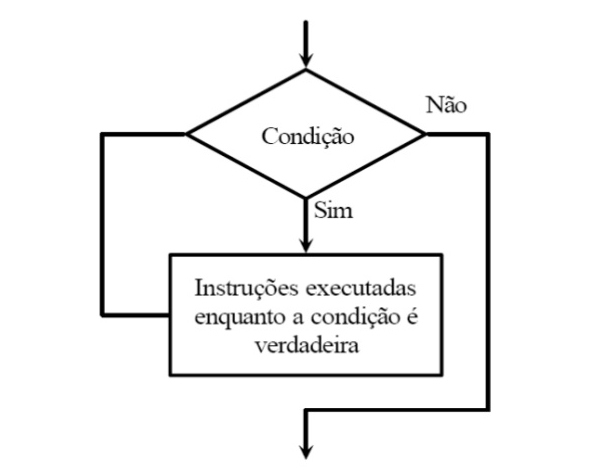
\includegraphics[width=0.5\textwidth]{img/laco-while.png}
    \caption{Fluxograma demonstrando um laço de repetição.}
    \label{fig:lacosimples}
  \end{center}
\end{figure}

Para demonstrar o uso desta estrutura de laço, apresentamos 3 exemplos simples. As soluções dos problemas serão demonstradas usando representação gráfica de fluxograma;  representação em Pseudocódigo; com Javascript e com Octave. 

\subsection{Problema~\ref{problema(while1)}}
\label{problema(while1)}
Escrever um algoritmo/programa para \emph{mostrar na tela os números de 1 até 10, usando repetição.}

\subsubsection{Fluxograma para solução do problema~\ref{problema(while1)}}
A Figura~\ref{fig:problema1} mostra um algoritmo, que resolve este problema, representado em fluxograma. 

Para resolver o problema criamos uma variável (i) com valor inicial 1; no losango representamos a verificação do laço, onde o algoritmo testa se a variávei i ainda é menor ou igual a 10; se i ainda é menor/igual a 10, o programa mostra o valor de i e faz com que a variável i receba o valor de i mais 1 (chamamos isso de incremento de variável). Caso o teste de i seja maior que 10, então o fluxo é desviado para o fim do programa.

\begin{figure}[h]
  \begin{center}
    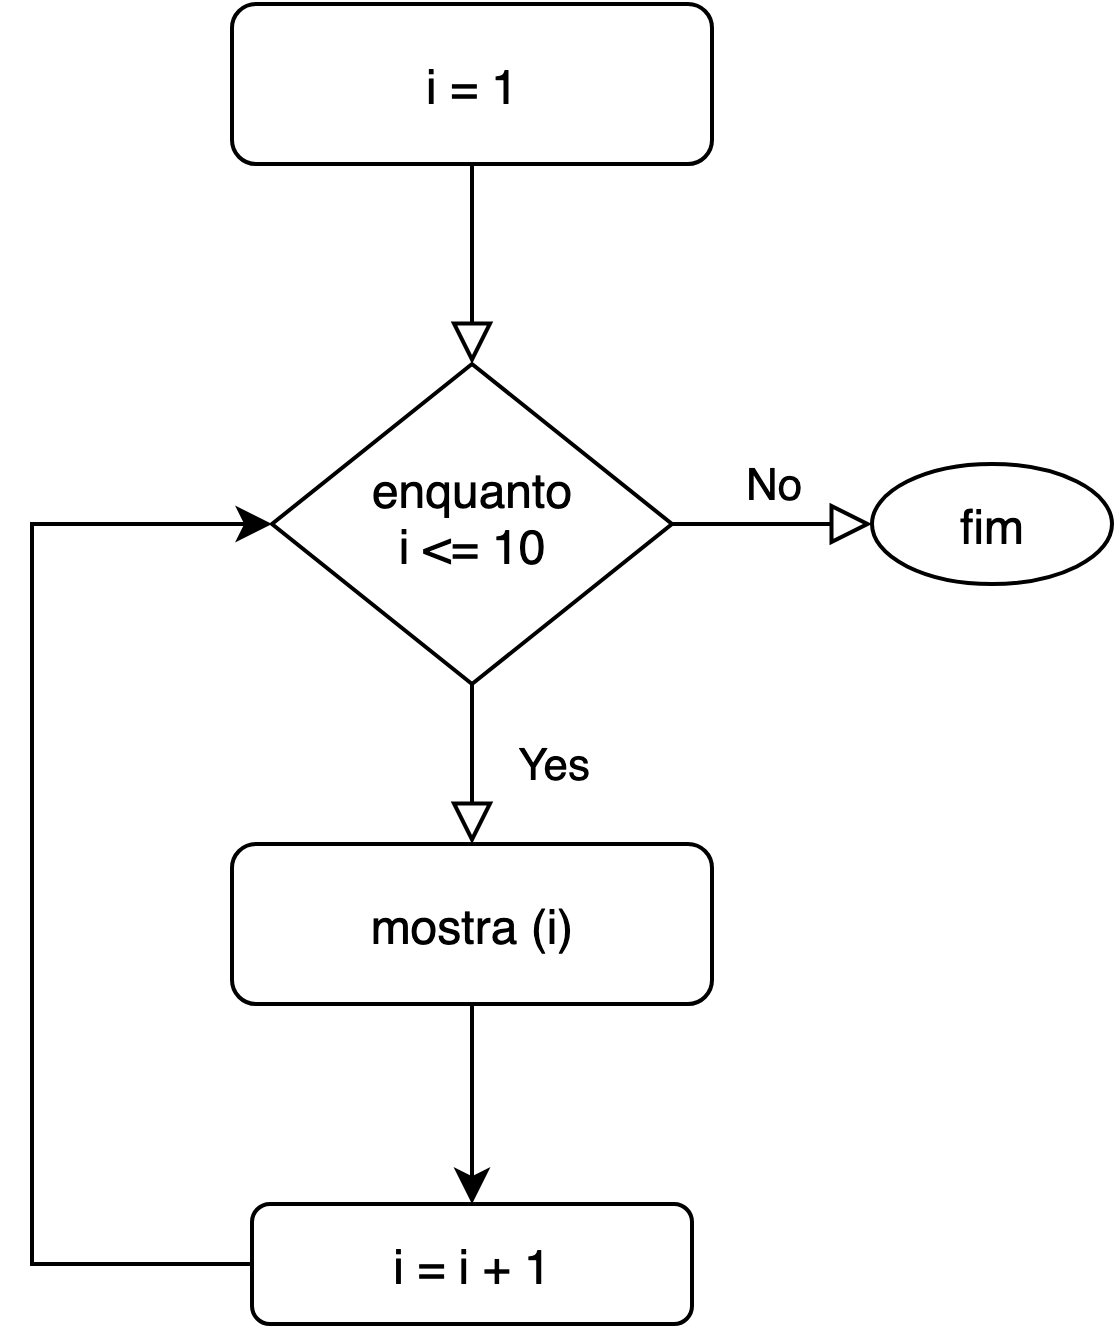
\includegraphics[width=0.5\linewidth]{img/problemaWhile1.png}
    \caption{Fluxograma representando a solução do problema~\ref{problema(while1)}.}
    \label{fig:problema1}
  \end{center}
\end{figure}

\subsubsection{Pseudocódigo}
Uma solução usando Pseudocódigo.
\begin{pseudocode}
Inicio
var i = 1
enquanto i <= 10, repita:
  mostra i
  i = i + 1
fim-enquanto
Fim 
\end{pseudocode}

\subsubsection{Javascript}
Uma solução usando JavaScript.
\begin{code}
var i = 1;
while(i <= 10){
  print(i);
  i = i + 1;
} 
\end{code}

\subsubsection{Octave}
Uma solução usando Octave. 
\begin{code}
clear
i = 1
while (i <= 10)
  printf(" %d ",i)
  i++
endwhile
\end{code}

Observe que a estrutura de uso da instrução while é semelhante nas linguagens JavaScript e Octave. No código em Octave, a instrução i++ é equivalente a instrução i = i+1.

Escolha uma das linguagens e execute o trecho observando o teste que ocorre dentro do parênteses. Observe também o resultado se tirarmos o sinal de “=” o laço repete de 1 até 9.


\subsection{Problema~\ref{problema(while2)}}
\label{problema(while2)}
Escrever um algoritmo/programa que leia 25 números, calculando e mostrando a média aritmética.

\subsubsection*{Fluxograma para solução do problema~\ref{problema(while2)}}
A Figura~\ref{fig:problema2} apresenta uma solução, na forma de fluxograma, para o problema~\ref{problema(while2)}.

\begin{figure}[h]
  \begin{center}
    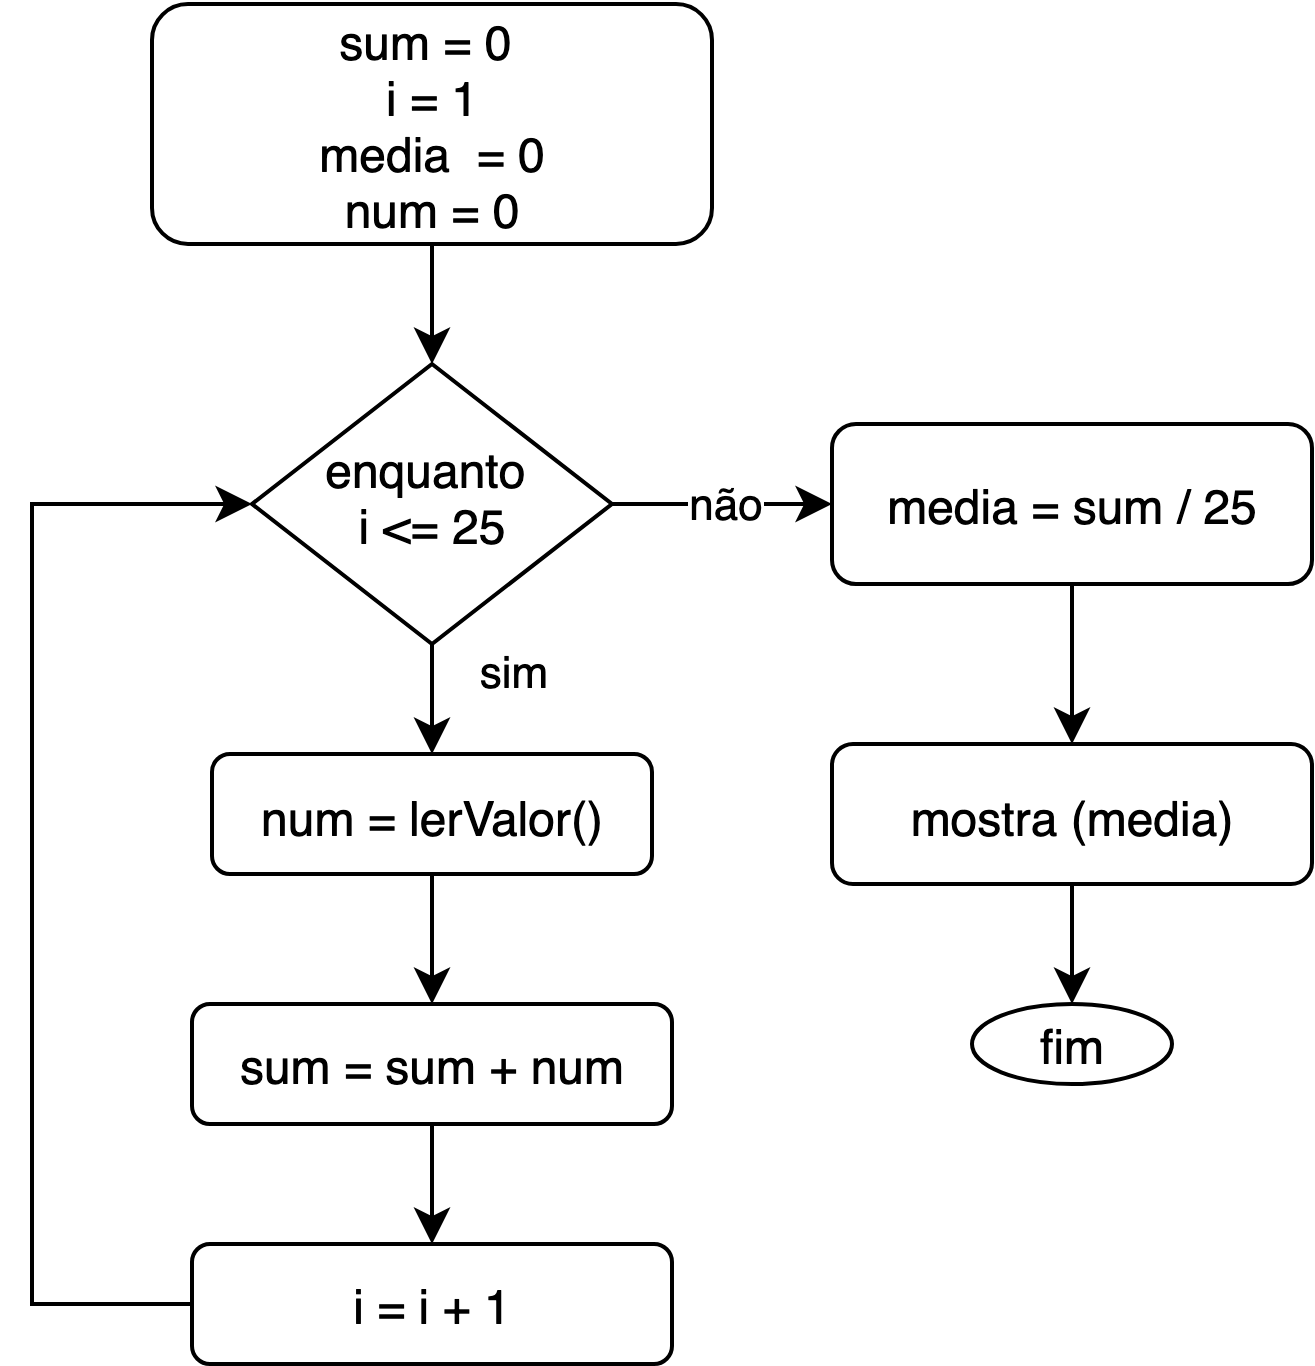
\includegraphics[width=0.5\linewidth]{img/problemaWhile2.png}
    \caption{Fluxograma representando a solução para o~\ref{problema(while2)}.}
    \label{fig:problema2}
  \end{center}
\end{figure}

No primeiro elemento do fluxograma, são definidas 4 variáveis, que são: 
\begin{itemize}
  \item $sum$, com valor 0. Esta variável será responsável por armazenar (acumular) o valor da soma dos números digitados.
  \item $i$, com valor 1. Esta variável servirá responsável pelo controle de quantas vezes o laço está sendo repetido. Lembrando que será necessário ler 25 números, portanto o laço vai precisar repetir pelo menos 25 vezes.
  \item $media$, com valor 0. Esta variável será usada para armazenar o cálculo da média.
  \item $num$, com valor 0. Esta variável será usada para armazenar cada valor lido. Importante, que cada valor lido, depois de somado pode ser descartado. Logo esta variável é reaproveitada a cada iteração do laço.
\end{itemize}

O losango representa o laço que executa enquanto i for menor ou igual a 25 (e que encerra quando i for maior que 25). 

Enquanto i for menor que 26, serão executados as instruções:
\begin{itemize}
  \item $num = lerValor()$; esta instrução lê um número digitado pelo teclado e armazena na variável num;
  \item $sum = sum + num$; esta instrução guarda em na variável sum, o valor de sum somado ao valor num;
  \item $i = i + 1$; esta instrução incrementa o valor de i para que se controle as 25 repetições dentro deste laço;
\end{itemize}

Uma outra forma de fazer analisar este algoritmo é usando uma tabela. Para isso, vamos observar a Tabela~\ref{tab:testemesa1}. Para não ficar muito longa, a tabela foi dividida ao meio montada lado a lado. Observe que a primeira coluna esta apenas dizendo se o programa ainda está dentro do laço - ele fica dentro do laço até que i=26. Cada linha da tabela, \texttt{enquanto o programa está dentro do laço}, é chamada de iteração. Os números na coluna num foram gerados aleatoriamente, simulando números que o usuário digitou. 

O valor na célula $sum$ é obtido conforme a equação $sum = sum + num$, ou seja, \texttt{o valor nela é sempre dado pela soma de sum da linha anterior com o valor num da linha corrente}. 

Vamos ver a iteração em que i=4: ao iniciar esta iteração, o valor de sum é 23. O usuário digitou 7 e como $sum = sum + num$, ao final da iteração sum recebe a soma entre o valor que tinha antes (no inicio da iteração) com o valor que o usuário acabou de digitar.

\begin{table}[h]
\caption{Um teste de mesa para a solução do problema~\ref{problema(while2)}.}
\begin{center}
\begin{tabular}{|c|c|c|c|c|c|c|c|c|c|c|}
\hline
\multicolumn{1}{|l|}{Laço} & \multicolumn{ 4}{c|}{Variáveis} & \multicolumn{1}{l|}{} & \multicolumn{1}{l|}{Laço} & \multicolumn{1}{l|}{} & \multicolumn{1}{l|}{} & \multicolumn{1}{l|}{} & \multicolumn{1}{l|}{} \\ \hline
dentro? & i & num & sum & media &  & dentro? & i & num & sum & media \\ \hline
sim & 0 & 0 & 0 & 0 &  & sim & 14 & 8 & 82 & 0 \\ \hline
sim & 1 & 10 & 10 & 0 &  & sim & 15 & 1 & 83 & 0 \\ \hline
sim & 2 & 5 & 15 & 0 &  & sim & 16 & 10 & 93 & 0 \\ \hline
sim & 3 & 8 & 23 & 0 &  & sim & 17 & 2 & 95 & 0 \\ \hline
sim & 4 & 7 & 30 & 0 &  & sim & 18 & 1 & 96 & 0 \\ \hline
sim & 5 & 10 & 40 & 0 &  & sim & 19 & 10 & 106 & 0 \\ \hline
sim & 6 & 3 & 43 & 0 &  & sim & 20 & 1 & 107 & 0 \\ \hline
sim & 7 & 4 & 47 & 0 &  & sim & 21 & 9 & 116 & 0 \\ \hline
sim & 8 & 8 & 55 & 0 &  & sim & 22 & 4 & 120 & 0 \\ \hline
sim & 9 & 4 & 59 & 0 &  & sim & 23 & 5 & 125 & 0 \\ \hline
sim & 10 & 6 & 65 & 0 &  & sim & 24 & 6 & 131 & 0 \\ \hline
sim & 11 & 3 & 68 & 0 &  & sim & 25 & 3 & 134 & 0 \\ \hline
sim & 12 & 2 & 70 & 0 &  & não & 26 & 3 & 137 & 5,48 \\ \hline
sim & 13 & 4 & 74 & 0 &  & \multicolumn{1}{l|}{} & \multicolumn{1}{l|}{} & \multicolumn{1}{l|}{} & \multicolumn{1}{l|}{} & \multicolumn{1}{l|}{} \\ \hline
\end{tabular}
\end{center}
\label{tab:testemesa1}
\end{table}

\emph{Importante:} Os valores das variáveis \texttt{somente são mostrados na tela} depois que o laço acaba e a média é calculada. A Tabela~\ref{tab:testemesa1} representa a memória usada pelo programa durante os passos da execução.

\subsubsection*{Pseudocódigo}
Um algoritmo em pseudocódigo.
\begin{pseudocode}
Inicio
var sum = 0, i = 1, num=0, media=0
enquanto i <= 25, repita:
	num = lerValor()
	sum = sum + num
	i = i + 1
fim-enquanto
media = sum / 25
mostra(media)
Fim
\end{pseudocode}

\subsubsection*{JavaScript}
Um programa em Javascript.
\begin{code}
var i = 1,sum = 0,num,media;
while( i <= 25){
  num = parseInt(prompt());
  sum = sum + num;
  i = i + 1;
}
media = sum / 25;
print(media);
\end{code}

\subsubsection*{Octave}
Um programa em Octave.
\begin{code}
clear
i = 1, sum = 0, num = 0, media = 0
while (i <= 5)
  num = input("digite um numero" )
  sum = sum + num
  i++
endwhile
media = sum / 5
printf(" %d ",media)
\end{code}


\subsection*{Problema~\ref{problema(while3)}}
\label{problema(while3)}
Escrever um algoritmo/programa para ler um uma quantidade variável (que muda) de valores e apresentar a média aritmética. 

Este problema poderia ser enunicado de outras formas, por exemplo:
\begin{enumerate}
  \item Ler N valores e apresentar a média aritmética na tela; ou
  \item Crie um programa que leia quantos números serão informados, depois leia estes números e faça a média.
\end{enumerate}

Para criar a solução para este problema é preciso compreender que cada vez que o programa executar, poderemos ler uma quantidade de valores diferentes. Por exemplo: usando o  mesmo programa quero fazer a média de notas da turma X (que tem 10 alunos) e em outro momento, quero fazer a média de notas dos alunos da turma Y (que tem 25 alunos). Para isso, precisamos de um programa que execute um laço de repetição de 1 até N, onde N é um valor informado pelo usuário.

\subsubsection*{Fluxograma para solução do problema~\ref{problema(while3)}}
A Figura~\ref{fig:fluxogramaproblema3} apresenta uma solução, na forma de fluxograma, para o problema~\ref{problema(while3)}.
\begin{figure}[h]
  \begin{center}
    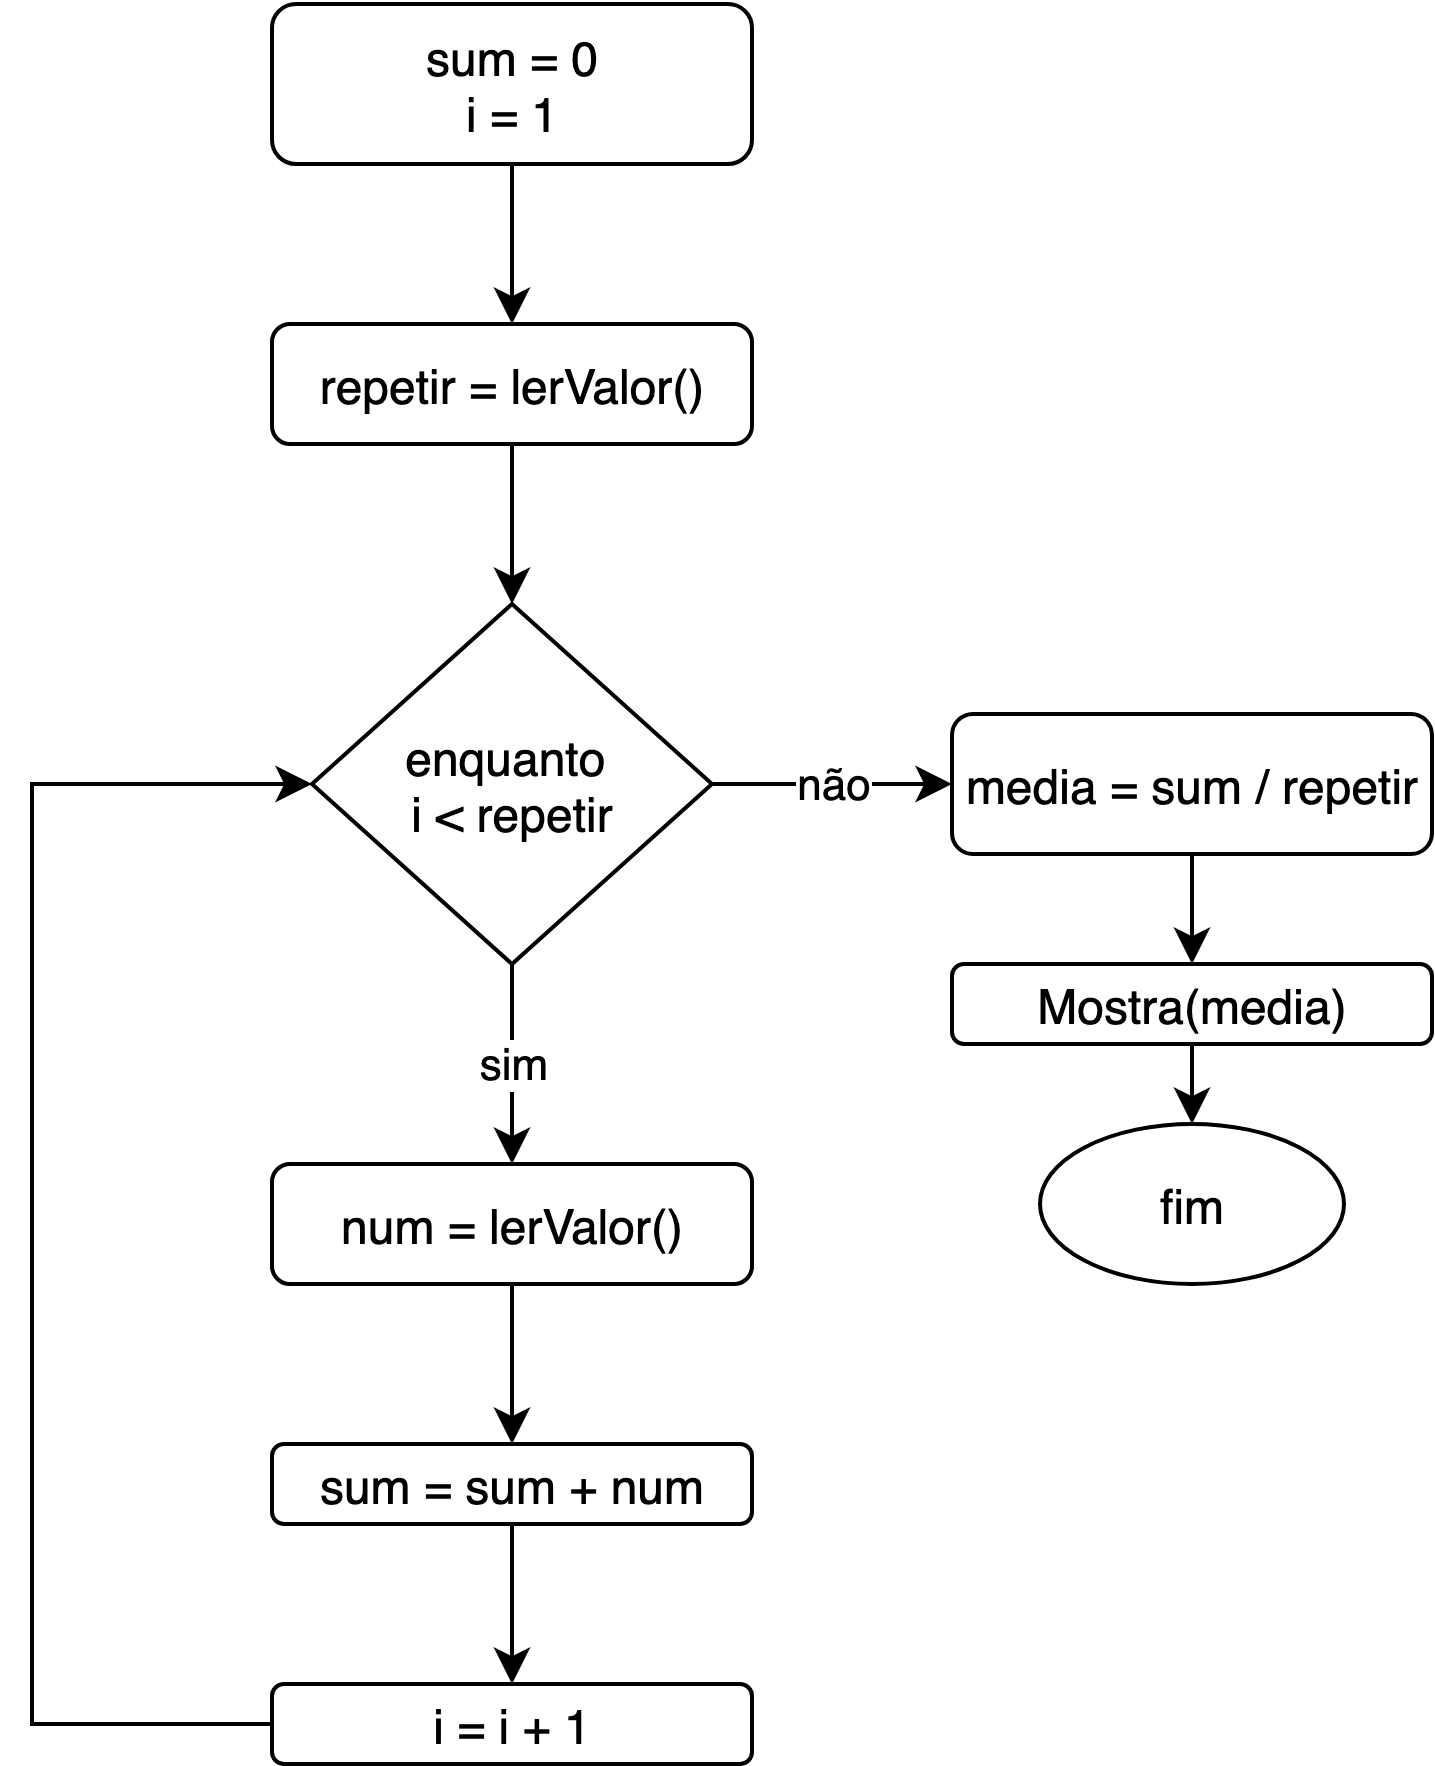
\includegraphics[width=0.5\linewidth]{img/problemaWhile3.png}
    \caption{Fluxograma representando a solução pra o problema~\ref{problema(while3)}.}
    \label{fig:fluxogramaproblema3}
  \end{center}
\end{figure}

Nesta solução iniciamos o algoritmo criando varáveis $sum$ com valor 0 e $i$ com valor 1. Na segunda ação, é criada a variável repetir com valor informado diretamente pelo teclado (esta variável irá determinar até quando o laço deverá repetir). 

O próximo passo, no losango, temos o controle do laço - veja que o laço diz: $enquanto i<repetir$, ou seja, enquanto a variável i (que iniciou em 1) for menor que a quantidade de valores que preciso ler ($repetir$). Enquanto $i$ for menor que $repetir$, o programa ficará preso no laço e fará:
\begin{itemize}
  \item $num = lerVavlor()$, que carrega em num um valor digitado pelo teclado;
  \item $sum = sum + num$, que soma na variável $sum$ todos valores digitados;
  \item $i = i + 1$, que incrementa o valor de $i$ em 1.
\end{itemize}

Este laço irá se repetir até que i não seja mais menor que repetir. Quando isto acontecer teremos somados todos os valores digitados pelo teclado.

Quando o laço encerrar, vamos para o fluxo da direita, onde é calculado a média em $media=sum/repetir$ e depois mostra a media na tela em $Mostra(media)$.

\subsubsection*{Pseudocódigo}
Uma solução em pseudocódigo.
\begin{pseudocode}
Inicio
var repetir, valor, media, i =0, sum = 0 ;
repetir = lerValor()
enquanto i < repetir, repita:
  valor = lerVAlor();
  i = i + 1;
sum = sum + valor;
fim-enquanto
media = sum/repetir
mostrar(media)
Fim
\end{pseudocode}

\subsubsection*{JavaScript}
Uma solução em JavaScript.
\begin{code}
var repetir, valor, media, i=1, sum = 0;

repetir = parseInt(prompt("Quantos numeros vc quer ler? "));
print(repetir)

while(i < repetir){
  valor = parseInt(prompt("Digite um valor: "));
  sum = sum + valor;
  i = i + 1;
}
media = sum / repetir;
print(media);
\end{code}

\subsubsection*{Octave}
Uma solução em Octave.
\begin{code}
clear

i = 1, sum = 0
repetir = input("Quantos numero quer ler? ")

while (i <= repetir)
  num = input("digite um numero" )
  sum = sum + num
  i++
endwhile
media = sum / repetir
printf(" %f ",media)
\end{code}


% ============================================ DO - WHILE ============================================ 
\section{Laço Do-While/Do-Until}
\label{sec:dowhile}

\begin{center}
  \emph{->-> O par de instruções do-while executa laços do tipo faça-enquanto <-<-}  
\end{center}

Nesta técnica executamos um conjunto de instrução enquanto uma determinada condição for verdadeira. O conjunto de instruções a ser repetido é executado ANTES do teste, sendo que este conjunto de instruções é executado pelo menos uma vez. 

Na técnica anterior~(\ref{sec:while}) o conjunto de instruções é executado DEPOIS do teste, podendo ocorrer situações em que não ocorra nenhuma execução deste bloco.

O diagrama apresentado na Figura~\ref{fig:laco-do-while}, mostra graficamente este tipo de repetição.

\begin{figure}[h]
  \begin{center}
    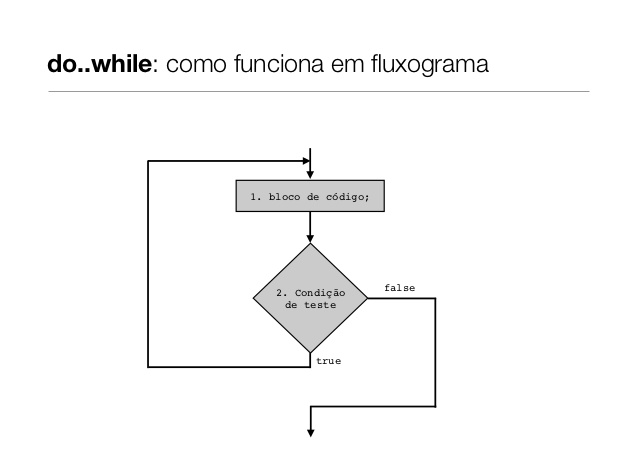
\includegraphics[width=0.75\linewidth]{img/laco-do-while.png}
    \caption{Fluxograma representando o funcionamento de um laço do tipo do-while.}
    \label{fig:laco-do-while}
  \end{center}
\end{figure}

\subsection{Problema~\ref{sec:problema(do-while1)}}
\label{sec:problema(do-while1)}

Escreva um algoritmo/programa que apresente na tela, a mensagem “continuar”, pelo menos uma vez, até que o valor -1 seja inserido no programa.

\subsubsection*{Fluxograma de uma solução para o problema~\ref{sec:problema(do-while1)} }
\begin{figure}[h]
  \begin{center}
    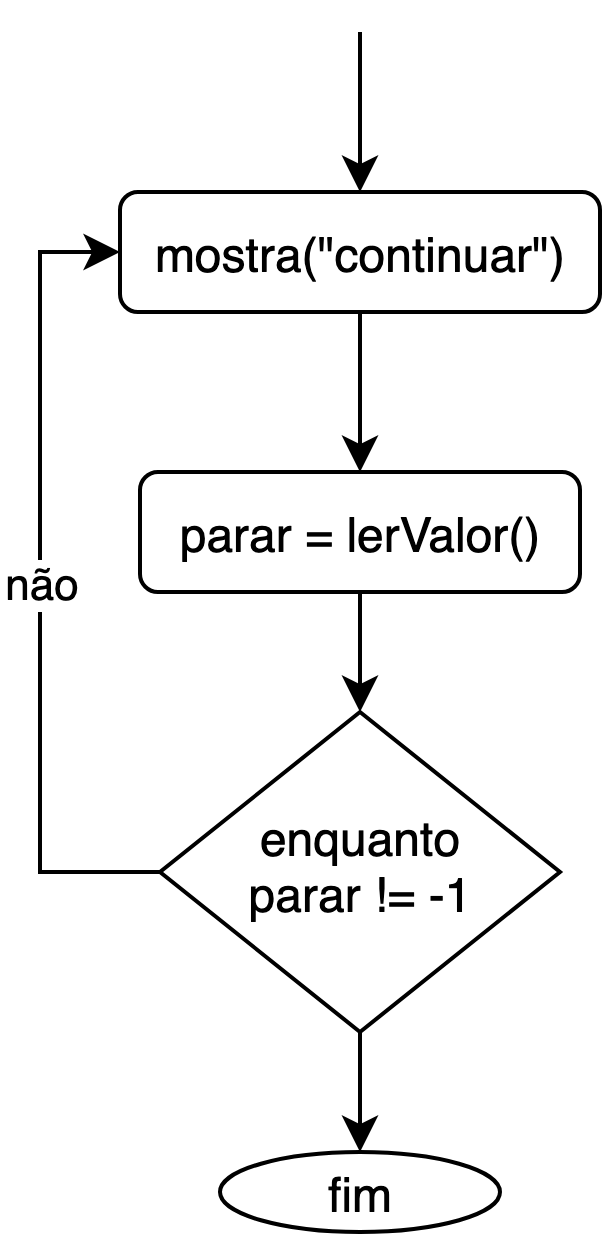
\includegraphics[width=0.4\linewidth]{img/problemaDoWhile1.png}
    \caption{Fluxograma representando a solução para o problema~\ref{sec:problema(do-while1)}.}
    \label{fig:problemaDoWhile1}
  \end{center}
\end{figure}

O laço inicia mostrando a palavra $continuar$. O segundo passo a ser feito é a leitura de um valor do teclado. Por fim, o teste do laço, que verifica que foi digitado $-1$: Se o teste for falso, retorno para o inicio do laço; se o teste deu verdadeiro então o programa vai para o fim.


\subsubsection*{Pseudocódigo}
Um algoritmo em pseudocódigo, que soluciona o problema~\ref{sec:problema(do-while1)}.
\begin{pseudocode}
Inicio
var parar;
faca
	mostrar("continuar");
	parar = lerValor();
enquanto (parar != -1)
Fim
\end{pseudocode}


\subsubsection*{JavaScript}
Um algoritmo em JavaScript, que soluciona o problema~\ref{sec:problema(do-while1)}.
\begin{code}
var parar;
do{
	print("continuar");
	parar = prompt("-1 finalizar / outro valor para continuar");
}
while(parar != -1);
\end{code}

\subsubsection*{Octave}
A linguagem Octave não dispõe de  um mecanismo faça-enquanto. Nesta linguagem utiliza-se um mecanismo chamado faça-até, executado pela instrução do-until. Na prática o que muda é apenas a forma com que o teste final é feito. 

O laço se encerra quando a condição for verdadeira (no faça-enquanto o laço se encerra quando a condição for falsa). 

Um algoritmo em Octave, que soluciona o problema~\ref{sec:problema(do-while1)} utilizando a técnica $do-until$.
\begin{code}
clear
do
  disp("Continuar....")
  parar = input("-1 para finalizar: ")
until(parar == -1)
\end{code}


\subsection{Problema~\ref{sec:problema(do-while2)}}
\label{sec:problema(do-while2)}

Usando a estrutura de laço do-while (ou do-until para Octave), criar um algoritmo/programa para apresentar os números ímpares de 1 até N, sendo N um valor estipulado pelo usuário.

\subsubsection*{Fluxograma}
\begin{figure}[h]
  \begin{center}
    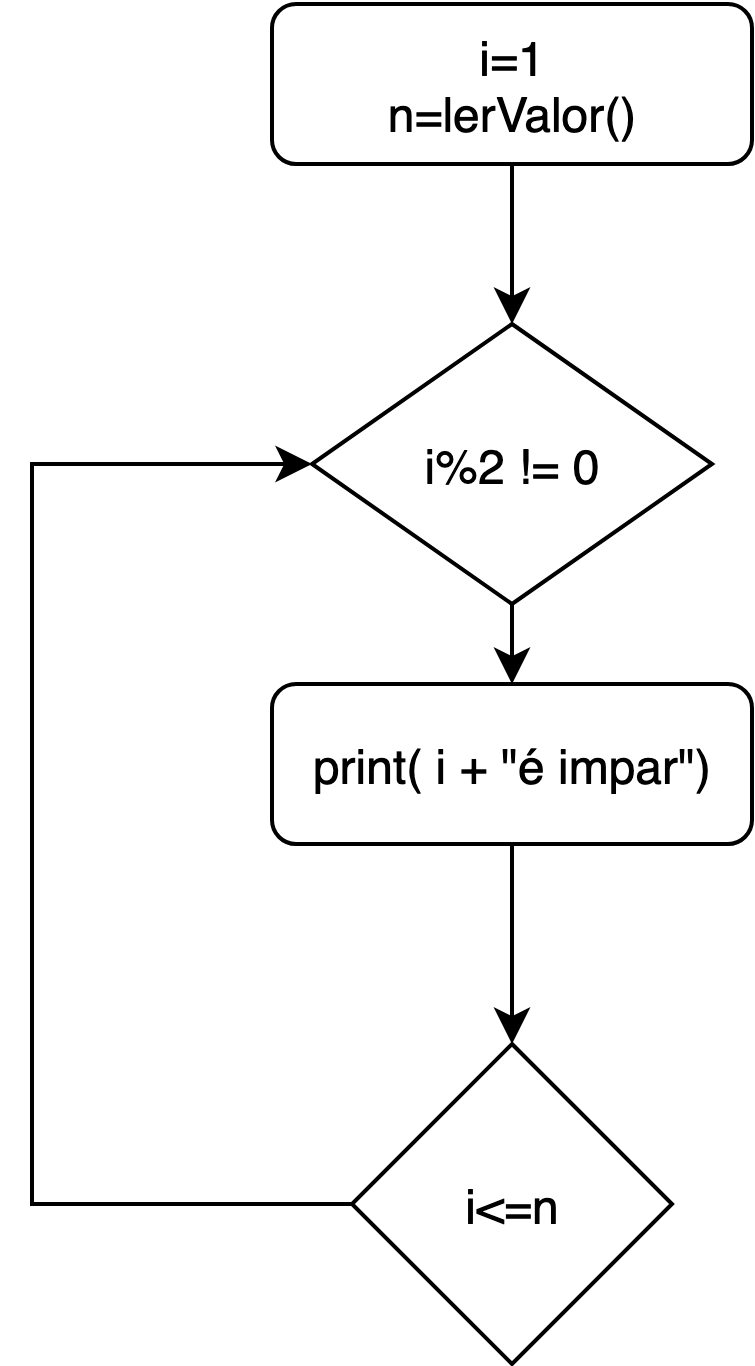
\includegraphics[width=0.4\linewidth]{img/problemaDoWhile2.png}
    \caption{Fluxograma representando a solução para o problema~\ref{sec:problema(do-while2)}.}
    \label{fig:problema(do-while2)}
  \end{center}
\end{figure}

\subsubsection*{Pseudocódigo}
Um algoritmo em pseudocódigo, que soluciona o problema ??.
\begin{pseudocode}
\end{pseudocode}


\subsubsection*{JavaScript}
Um algoritmo em JavaScript, que soluciona o problema ??.
\begin{code}
\end{code}

\subsubsection*{Octave}
Um algoritmo em Octave, que soluciona o problema ??.
\begin{code}
\end{code}



% ============================================ GENERICO ============================================ 
\section{Tipo de laço}
\label{sec:tipolaco}

\subsection{Problema ??}
\label{sec:problema?}

\subsubsection*{Fluxograma}
\begin{figure}[h]
  \begin{center}
    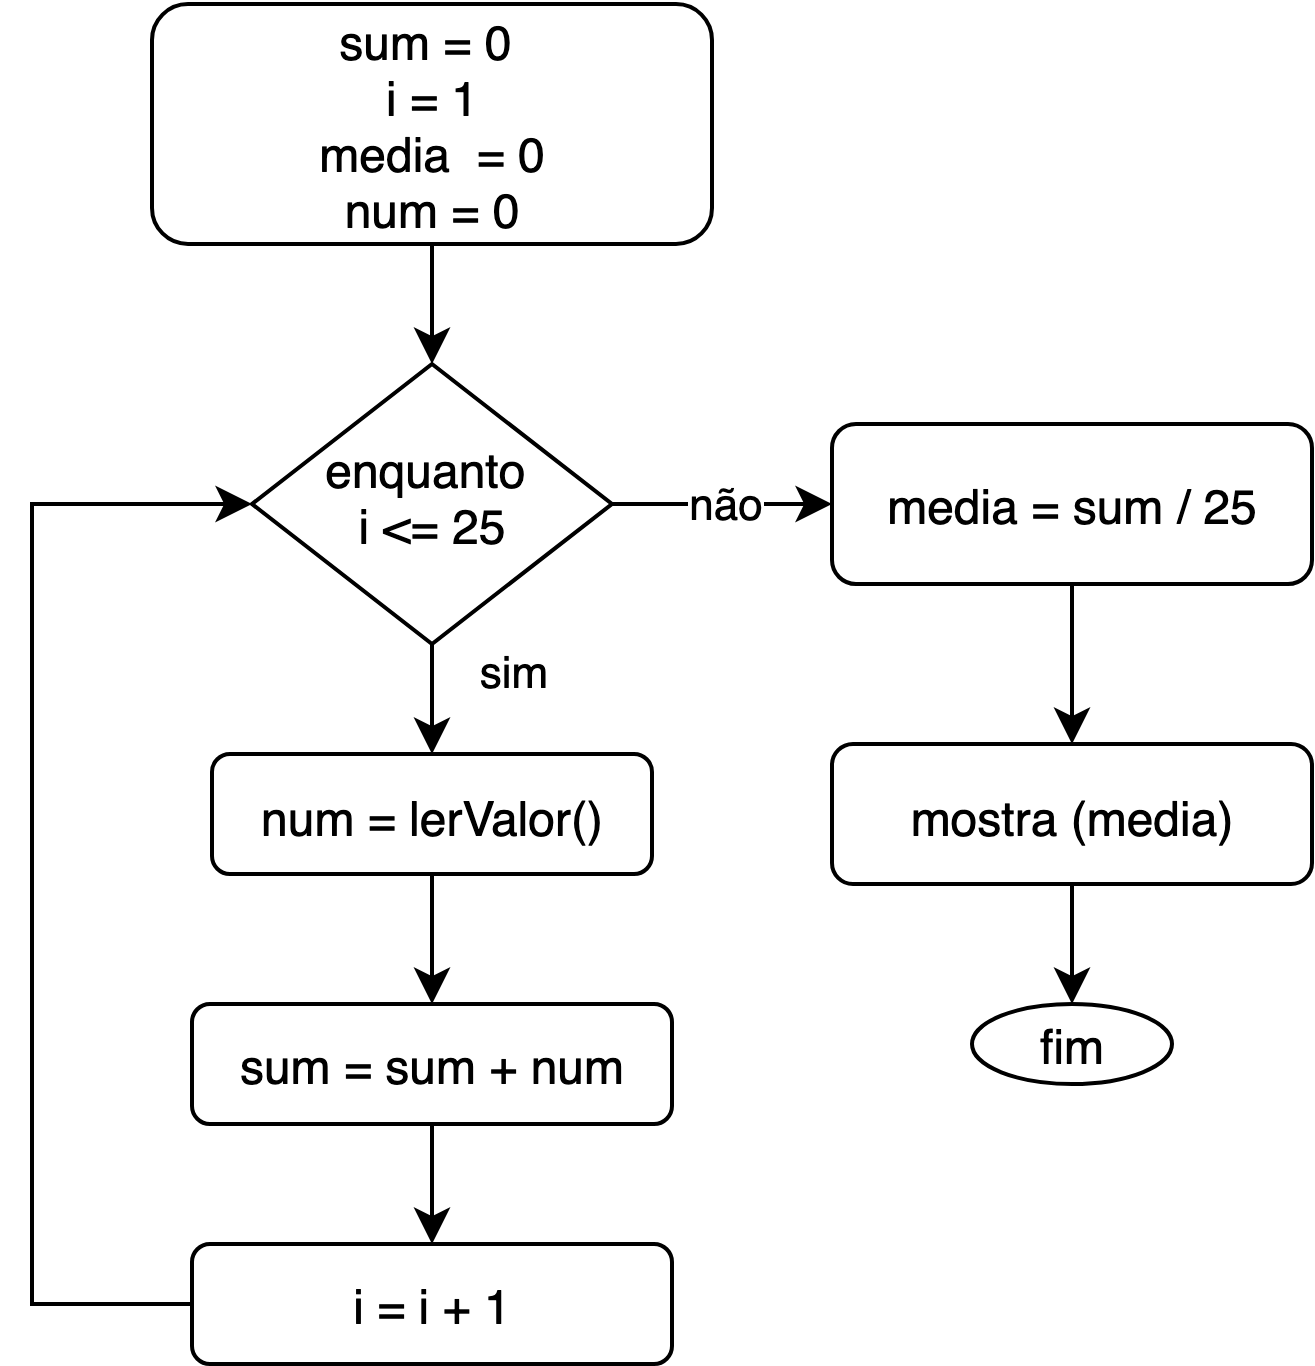
\includegraphics[width=0.5\linewidth]{img/problemaWhile2.png}
    \caption{Fluxograma representando a solução para o problema ???.}
    \label{fig:problema???}
  \end{center}
\end{figure}

\subsubsection*{Pseudocódigo}
Um algoritmo em pseudocódigo, que soluciona o problema ??.
\begin{pseudocode}
\end{pseudocode}


\subsubsection*{JavaScript}
Um algoritmo em JavaScript, que soluciona o problema ??.
\begin{code}
\end{code}

\subsubsection*{Octave}
Um algoritmo em Octave, que soluciona o problema ??.
\begin{code}
\end{code}
